\documentclass[12pt,a4paper,twoside,twocolumn]{article}

%% isso ficou obsoleto -- desde 2020 o compilador usa utf8
% \usepackage[utf8]{inputenc}

%% Margens
%% NOTA: o uso das margens aqui (margens diferentes p/ frente e verso) está meio que assumindo que a primeira página é uma página da frente, e que o caderno seria grampeado na lateral inteira (tipo o do ENEM). Se só for grampeado na ponta, as margens seriam diferentes.
\usepackage[top=2cm, bottom=2cm, left=1.5cm, right=1.2cm]{geometry}
\usepackage[brazil]{babel}
\newcommand{\sen}{\operatorname{sen}}

%% Separador entre colunas
\setlength{\columnseprule}{0.4pt}
\setlength{\columnsep}{6mm}

%%% Varias colunas
\usepackage{multicol}

%%% Referência à última página
\usepackage{lastpage}

%%% Matemática
\usepackage{amsmath}

%%% Fonte sem serifa
\usepackage{lmodern}
\usepackage{sansmathfonts}
\renewcommand*{\familydefault}{\sfdefault}

%%% Imagens
\usepackage{graphicx}

%%% Cabeçalho e rodapé
\usepackage{fancyhdr}
\pagestyle{fancy}
\fancyhf{}

% Cabeçalho
\fancyhead[C]{
\includegraphics[height=8mm]{images/logo-simulado.png}}

% Rodapé
\fancyfoot[LE,RO]{\thepage~de~\pageref{LastPage}}
\fancyfoot[C]{\small Simulado Emancipa -- Caderno único}
\fancyfoot[RE,LO]{\small 
\includegraphics[height=12pt]{images/logo-simulado.png}}

%%% Questão
\usepackage{enumitem}
\usepackage{tikz}

\newcounter{questao}
\setcounter{questao}{0} 
\definecolor{qgray}{gray}{0.85}
\newcommand{\questao}{
  \refstepcounter{questao}
  \noindent\textbf{\footnotesize QUESTÃO \arabic{questao}}
  \textcolor{qgray}{\hspace{2ex}\leaders\vrule height 8pt depth -0.1pt \hfill \null}
  \par
  \nopagebreak
  \vspace{-8pt}
  \noindent\rule[3pt]{\columnwidth}{1pt}
  \nopagebreak
}

% Circula alguma letra
\newcommand*{\circled}[1]{%
  \tikz[baseline=(char.base)]{
    \node[
      shape=circle,
      fill,
      text=white,
      font=\bfseries,
      inner sep=0.5pt
    ] (char) {#1};
  }
}

% Alternativas
\newenvironment{alternativas}{%
  \begin{enumerate}[
    label=\protect\circled{\scriptsize\Alph*},
    leftmargin=8mm,
    itemsep=-3pt,
    topsep=1ex
    ]
  }{%
  \end{enumerate}
}

% Citação
\newcommand{\citacao}[2]{
    #1
    \vspace{-1ex}
    \begin{flushright}
    \scriptsize
    #2
    \end{flushright}
}

\usepackage{lipsum} % for some dummy text

\begin{document}

\noindent{\small\textbf{LINGUAGENS, CÓDIGOS E SUAS TECNOLOGIAS}}

\noindent\textbf{Questões 1 a \ref{last-linguagens}} %arrumar o número
\medskip

% (ENEM - 2018 - PROVA AMARELA)
\questao
\vspace{-\baselineskip}
\citacao{
\begin{verse}
Don't write in English, they said, \\
English is not your mother tongue\dots \\
\dots The language I speak \\
Becomes mine, its distortions, its queerness \\
All mine, mine alone, it is half English, half \\
Indian, funny perhaps, but it is honest, \\
It is as human as I am human\dots \\
\dots It voices my joys, my longings my \\
Hopes\dots

(Kamala Das, 1965:10)
\end{verse}
}{GARGESH, R. South Asian Englishes. In: KACHRU, Y; NELSON, C. L. (Eds.). The Handbook of World English. Singapore: Blackwell, 2006}
A poetisa Kamala Das, como muitos escritores indianos, escreve suas obras em inglês, apesar de essa não ser sua primeira língua. Nesses versos, ela
\begin{alternativas}
\item usa a língua inglesa como efeito humorístico.
\item recorre a vozes de vários escritores ingleses.
\item adverte sobre o uso distorcido da língua inglesa.
\item demonstra consciência de sua identidade linguística.
\item reconhece a incompreensão na sua maneira de falar inglês.
\end{alternativas}

% (ENEM - 2019 - PROVA AMARELA)

\questao
\citacao{
  \begin{verse}
    Is this life \\
    Sitting on a park bench \\
    Thinking about a friend of mine \\
    He was only twenty-three \\
    Gone before he had his time \\
    It came without a warning \\
    Didn’t want his friend to see him cry \\
    he knew the day was dawning \\
    And I didn’t have a chance to say goodbye \\
  \end{verse}
} {
  MADONNA. Erotica. Estados Unidos. Marverick, 1992.
}

A canção, muitas vezes, é uma forma de manifestar sentimentos e emoções da vida cotidiana. Por exemplo, o sofrimento retratado nessa canção foi causado:

\begin{alternativas}
  \item pela morte precoce de um amigo jovem.
  \item pelo término de um relacionamento amoroso.
  \item pela mudança de um amigo para outro país.
  \item pelo fim de uma amizade de mais de vinte anos.
  \item pela traição por parte de pessoa próxima.
\end{alternativas}

% (UNICAMP- SP - 2019)Número Original: 84Código: 6983669

\questao
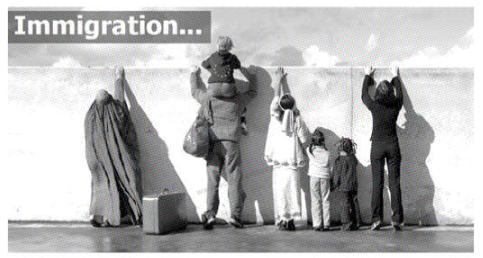
\includegraphics[width=\columnwidth]{subareas/linguagens/ingles-1.png}
\citacao{
  Your Car is German. Your Vodka is Russian. Your Pizza is Italian.
  Your Democracy is Greek. Your Coffee is Brazilian. Your Movies are
  American. Your Shirt is Indian. Your Oil is Saudi Arabian. Your
  Electronics are Chinese. Your Numbers Arabic, your Letters Latin.
  And YOU complain that YOUR Neighbor is an Immigrant?
} {
  (Adaptado de https://br.pinterest.com. Acessado em 10/06/2018.)
}
O post anterior aponta
\begin{alternativas}
  \item as vantagens da globalização para o consumidor e os problemas causados pela imigração.
  \item o impacto negativo dos processos migratórios no modo como as culturas vêm sendo globalizadas.
  \item os efeitos da globalização no nosso cotidiano e o preconceito contra imigrantes.
  \item o consumo excessivo de produtos estrangeiros no mundo capitalista contemporâneo.
\end{alternativas}

% (UNICAMP- SP - 2019)Número Original: 87Código: 6983667

\questao
\begin{center}

\includegraphics[width=0.6\columnwidth]{subareas/linguagens/ingles-4.png}
\end{center}
Os dizeres da camiseta:
\begin{alternativas}
  \item brincam com palavras do inglês que têm grafias e pronúncias semelhantes.
  \item criam um efeito de humor explorando a ambiguidade de certas palavras do inglês.
  \item brincam com o fato de o inglês ser uma língua irracional e incompreensível.
  \item criam um efeito de humor a partir da complexidade do sistema ortográfico do inglês.
\end{alternativas}

% (UNESP - 2021)Número Original: 27Código: 9363635

\questao
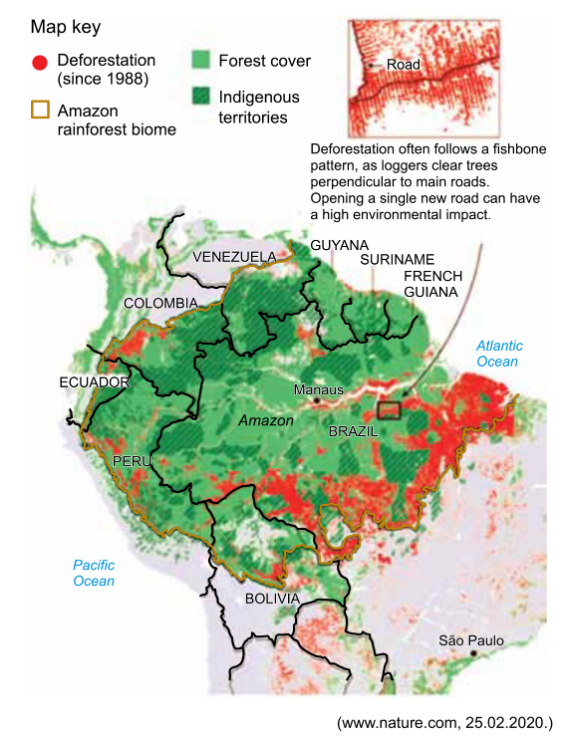
\includegraphics[width=\columnwidth]{subareas/linguagens/ingles-2.png}
The country covered by the Amazon rainforest presented in the map that displays less signs of forest clearing is:
\begin{alternativas}
  \item Ecuador.
  \item Colombia.
  \item Peru.
  \item French Guiana.
  \item Bolivia.
\end{alternativas}


% ENEM - 2021

\questao
\citacao{
  We are now a nation obsessed with the cult of celebrity. Celebrities have replaced the classic notion of the hero. But instead of being respected for talent, courage or intelligence, it is money, style and image the deciding factors in what commands respect. Image is everything. Their image is painstakingly constructed by a multitude of different image consultants to carve out the most profitable celebrity they can. Then society is right behind them, believing in everything that celebrity believes in. Companies know that people will buy a product if a celebrity has it too. It is as if the person buying the product feels that they now have some kind of connection with the celebrity and that some of their perceived happiness will now be passed onto the consumer. So to look at it one way, the cult of celebrity is really nothing more than a sophisticated marketing scheme. Celebrities though cannot be blamed for all negative aspects of society. In reality society is to blame. We are the people who seemed to have lost the ability to think for ourselves. I suppose it's easier to be told what to think, rather than challenging what we are told. The reason we are swamped by celebrity is because there is a demand for it.
} {
  Disponível em: www. pitlanemagazine.com. Acesso em: 7 dez. 2017 (adaptado).
}

O texto, que aborda questões referentes ao tema do culto à celebridade, tem o objetivo de

\begin{alternativas}
  \item destacar os méritos das celebridades.
  \item criticar o consumismo das celebridades.
  \item ressaltar a necessidade de reflexão dos fãs.
  \item culpas as celebridades pela obsessão dos fãs.
  \item valorizar o marketing pessoal das celebridades
\end{alternativas}

% [PUCPR 2003]

\questao
Supply the sentences with the correct alternative: 

\begin{enumerate}[label=\Roman*., noitemsep, topsep=1ex]
\item  This is the hardest problem \rule{1cm}{1pt} I have ever had to face. 
\item  A doctor, \rule{1cm}{1pt} patients trust him, has great responsibility. 
\item  Vesuvius, \rule{1cm}{1pt} is a lofty volcano, overlooks the Bay of Naples. 
\item  My friend Marcello, \rule{1cm}{1pt} is in hospital, is very ill. 
\item  There's something \rule{1cm}{1pt} I must tell you in confidence.
\end{enumerate}

\begin{alternativas}
  \item I. that; II. which; III. what; IV. who; V. that 
  \item I. which; II. whose; III. that; IV. whose; V. which 
  \item I. that; II. whose; III. which; IV. who; V. that 
  \item I. what; II. who; III. which; IV. that; V. what 
  \item I. that; II. whose; III. what; IV. which; V. that
\end{alternativas}

\separador
\noindent A imagem abaixo será usada nas questões \textbf{\ref{ing1}}, \textbf{\ref{ing2}} e \textbf{\ref{ing3}}.
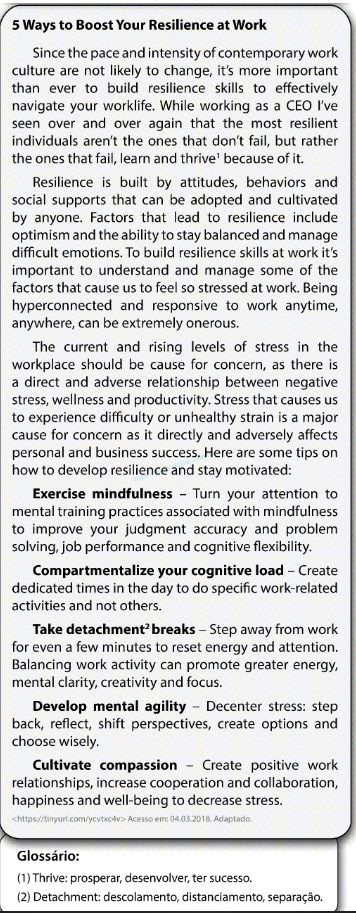
\includegraphics[width=\columnwidth]{subareas/linguagens/ingles-3.png}

\questao\label{ing1}
Segundo o texto, o crescente nível de estresse no trabalho
\begin{alternativas}
  \item deve ser motivo de preocupação pela pressão gerada.
  \item possibilita a cooperação e colaboração entre os trabalhadores.
  \item causa pressão favorável à busca por bem-estar e produtividade.
  \item estimula o trabalhador a buscar seu sucesso pessoal e profissional.
  \item cria competitividade e, consequentemente, aumenta a produtividade.
\end{alternativas}

\questao\label{ing2}
De acordo com o texto, a resiliência no mundo do trabalho
\begin{alternativas}
  \item é uma habilidade que poucas pessoas conseguem cultivar.
  \item está diretamente ligada a adversidades, causando o estresse.
  \item estabelece uma relação direta entre estresse negativo, bem-estar e produtividade.
  \item é desenvolvida com a compreensão e gerenciamento de fatores que nos causam estresse.
  \item é o resultado de um comportamento de constante conexão e disponibilidade para o trabalho.
\end{alternativas}

\questao\label{ing3}
No segundo parágrafo do texto o trecho ``... can be extremely onerous.'' refere-se a
\begin{alternativas}
  \item desenvolver a resiliência no trabalho.
  \item aumentar o nível de estresse no trabalho.
  \item estabelecer pausas excessivas durante o trabalho.
  \item compreender os fatores causadores do estresse no trabalho.
  \item estar constantemente conectado e disponível às demandas do trabalho.
\end{alternativas}


% 1.(Enem/2013)
\questao
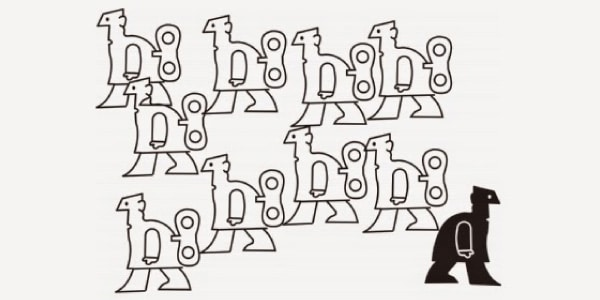
\includegraphics[width=\columnwidth]{subareas/linguagens/image3.png}
O cartum faz uma crítica social. A figura destacada está em oposição às outras e representa a
\begin{alternativas}
  \item a opressão das minorias sociais.
  \item carência de recursos tecnológicos.
  \item falta de liberdade de expressão.
  \item defesa da qualificação profissional.
\end{alternativas}

% 2.(Enem/2016)
\questao
\citacao{
  \begin{verse}
    Antiode

    Poesia, não será esse \\
    o sentido em que \\
    ainda te escrevo: \\
    flor! (Te escrevo: \\
    flor! Não uma \\
    flor, nem aquela \\
    flor-Virtude – em disfarçados urinóis). \\
    Flor é a palavra \\
    flor; verso inscrito \\
    no verso, como as \\
    manhãs no tempo. \\
    Flor é o salto \\
    da ave para o voo: \\
    o salto fora do sono \\
    quando seu tecido \\
    se rompe; é uma explosão \\
    posta a funcionar, \\
    como uma máquina, \\
    uma jarra de flores.
  \end{verse}
} {
  MELO NETO, J. C. Psicologia da composição Rio de Janeiro Nova Fronteira, 1997 (fragmento)
}
A poesia é marcada pela recriação do objeto por meio da linguagem, sem necessariamente explicá-lo. Nesse fragmento de João Cabral de Melo Neto, poeta da geração de 1945, o sujeito lírico propõe a recriação poética de
\begin{alternativas}
  \item uma palavra, a partir de imagens com as quais ela pode ser comparada, a fim de assumir novos significados.
  \item um urinol, em referência às artes visuais ligadas às vanguardas do início do século XX.
  \item uma ave, que compõe, com seus movimentos, uma imagem historicamente ligada à palavra poética.
  \item uma máquina, levando em consideração a relevância do discurso técnico-científico pós-Revolução Industrial.
  \item um tecido, visto que sua composição depende de elementos intrínsecos ao eu lírico.
\end{alternativas}

% 3.(Enem/2013)
\questao
\citacao{
  O jogo é uma atividade ou ocupação voluntária, exercida dentro de certos e determinados limites de tempo e de espaço, segundo regras livremente consentidas, mas absolutamente obrigatórias, dotado de um fim em si mesmo, acompanhado de um sentimento de tensão e de alegria e de uma consciência de ser diferente da ``vida quotidiana''.
} {
  HUIZINGA, J. Homo ludens: o jogo como elemento da cultura. São Paulo: Perspectiva, 2004.
}
Segundo o texto, o jogo comporta a possibilidade de fruição. Do ponto de vista das práticas corporais, essa fruição se estabelece por meio do(a)
\begin{alternativas}
  \item fixação de táticas, que define a padronização para maior alcance popular.
  \item competitividade, que impulsiona o interesse pelo sucesso.
  \item refinamento técnico, que gera resultados satisfatórios.
  \item caráter lúdico, que permite experiências inusitadas.
  \item uso tecnológico, que amplia as opções de lazer.
\end{alternativas}

% 4.(Enem/2014)
% 
\questao
\citacao{
  \noindent Censura moralista

  Há tempos que a leitura está em pauta. E, diz-se, em crise. Comenta-se esta crise, por exemplo, apontando a precariedade das práticas de leitura, lamentando a falta de familiaridade dos jovens com livros, reclamando da falta de bibliotecas em tantos municípios, do preço dos livros em livrarias, num nunca acabar de problemas e de carências. Mas, de um tempo para cá, pesquisas acadêmicas vêm dizendo que talvez não seja exatamente assim, que brasileiros leem, sim, só que leem livros que as pesquisas tradicionais não levam em conta. E, também de um tempo para cá, políticas educacionais têm tomado a peito investir em livros e em leitura.
} {
  LAJOLO, M. Disponível em: www.estadao.com.br. Acesso em: 2 dez. 2013 (fragmento).
}
Os falantes, nos textos que produzem, sejam orais ou escritos, posicionam-se frente a assuntos que geram consenso ou despertam polêmica. No texto, a autora
\begin{alternativas}
  \item ressalta a importância de os professores incentivarem os jovens às práticas de leitura.
  \item critica pesquisas tradicionais que atribuem a falta de leitura à precariedade de bibliotecas.
  \item rebate a ideia de que as políticas educacionais são eficazes no combate à crise de leitura.
  \item questiona a existência de uma crise de leitura com base nos dados de pesquisas acadêmicas.
  \item atribui a crise da leitura à falta de incentivos e ao desinteresse dos jovens por livros de qualidade.
\end{alternativas}

% 5.(Enem/2017)

\questao
\citacao{
  Essas moças tinham o vezo de afirmar o contrário do que desejavam. Notei a singularidade quando principiaram a elogiar o meu paletó cor de macaco. Examinavam-no sérias, achavam o pano e os aviamentos de qualidade superior, o feitio admirável. Envaideci-me: nunca havia reparado em tais vantagens. Mas os gabas se prolongaram, trouxeram-me desconfiança. Percebi afinal que elas zombavam e não me susceptibilizei. Longe disso: achei curiosa aquela maneira de falar pelo avesso, diferente das grosserias a que me habituara. Em geral me diziam com franqueza que a roupa não me assentava no corpo, sobrava nos sovacos.
} {
  RAMOS, G. Infância. Rio de Janeiro: Record, 1994.
}
Por meio de recursos linguísticos, os textos mobilizam estratégias para introduzir e retomar ideias, promovendo a progressão do tema. No fragmento transcrito, um novo aspecto do tema é introduzido pela expressão
\begin{alternativas}
  \item ``a singularidade''.
  \item ``tais vantagens''.
  \item ``os gabas''.
  \item ``Longe disso''.
  \item ``Em geral''.
\end{alternativas}
% 6.(Enem/2013)

\questao
\citacao{
  \noindent Novas tecnologias

  Atualmente, prevalece na mídia um discurso de exaltação das novas tecnologias, principalmente aquelas ligadas às atividades de telecomunicações. Expressões frequentes como ``o futuro já chegou'', ``maravilhas tecnológicas'' e ``conexão total com o mundo'',  ``fetichizam'' novos produtos, transformando-os em objetos do desejo, de consumo obrigatório. Por esse motivo carregamos hoje nos bolsos, bolsas e mochilas o ``futuro'' tão festejado. Todavia, não podemos reduzir-nos a meras vítimas de um aparelho midiático perverso, ou de um aparelho capitalista controlador. Há perversão, certamente, e controle, sem sombra de dúvida. Entretanto, desenvolvemos uma relação simbiótica de dependência mútua com os veículos de comunicação, que se estreita a cada imagem compartilhada e a cada dossiê pessoal transformado em objeto público de entretenimento. Não mais como aqueles acorrentados na caverna de Platão, somos livres para nos aprisionar, por espontânea vontade, a esta relação sadomasoquista com as estruturas midiáticas, na qual tanto controlamos quanto somos controlados.
} {
  SAMPAIO A. S. A microfísica do espetáculo. Disponível em: http://observatoriodaimprensa.com. br. Acesso em: 1 mar 2013 (adaptado).
}
Ao escrever um artigo de opinião, o produtor precisa criar uma base de orientação linguística que permita alcançar os leitores e convencê-los com relação ao ponto de vista defendido. Diante disso, nesse texto, a escolha das formas verbais em destaque objetiva
\begin{alternativas}
  \item criar relação de subordinação entre leitor e autor, já que ambos usam as novas tecnologias.
  \item enfatizar a probabilidade de que toda população brasileira esteja aprisionada às novas tecnologias.
  \item indicar, de forma clara, o ponto de vista de que hoje as pessoas são controladas pelas novas tecnologias.
  \item tornar o leitor copartícipe do ponto de vista de que ele manipula as novas tecnologias e por elas é manipulado.
  \item demonstrar ao leitor sua parcela de responsabilidade por deixar que as novas tecnologias controlem as pessoas. 
\end{alternativas}

% 7.(Enem/2013)


\questao

\includegraphics[width=\columnwidth]{subareas/linguagens/image2.png}
Nessa charge, o recurso morfossintático que colabora para o efeito de humor está indicado pelo(a)
\begin{alternativas}
  \item emprego de uma oração adversativa, que orienta a quebra da expectativa ao final.
  \item uso de conjunção aditiva, que cria uma relação de causa e efeito entre as ações.
  \item retomada do substantivo ``mãe'', que desfaz a ambiguidade dos sentidos a ele atribuídos.
  \item utilização da forma pronominal ``la'', que reflete um tratamento formal do filho em relação à ``mãe''.
  \item repetição da forma verbal ``é'', que reforça a relação de adição existente entre as orações.
\end{alternativas}

% 8.(Enem/2021)

\questao
\citacao{
  O documentário O menino que fez um museu, direção de Sérgio Utsch, produção independente de brasileiros e britânicos, gravado no Nordeste em 2016, mais precisamente no distrito Dom Quintino, zona rural do Crato foi premiado em Londres, pela Foreign Press Association (FPA), a associação de correspondentes estrangeiros mais antiga do mundo, fundada em 1888.

  De acordo com o diretor, O menino que fez um museu foi o único trabalho produzido por equipes fora do eixo Estados Unidos-Europa entre os finalistas. O documentário conta a história de um Brasil profundo, desconhecido até mesmo por muitos brasileiros. É apresentado com o carisma de Pedro Lucas Feitosa, 11 anos.

  Quando tinha 10 anos, Pedro Lucas criou o Museu de Luiz Gonzaga, que fica no distrito de Dom Quintino. A ideia surgiu após uma visita que o garoto fez, em 2013, quando tinha 8 anos, ao Museu do Gonzagão, em Exu, Pernambuco. Pedro decidiu criar o próprio lugar de exposição para homenagear o rei e o local escolhido foi a casa da sua bisavó já falecida, que fica ao lado da casa dele, na rua Alto de Antena.
}{}

No segundo parágrafo, uma citação afirma que o documentário "foi o único trabalho produzido por equipes fora do eixo Estados Unidos-Europa entre os finalistas". No texto, esse recurso expressa uma estratégia argumentativa que reforça a
\begin{alternativas}
  \item originalidade da iniciativa de homenagem à vida e à obra de Luiz Gonzaga
  \item falta de concorrentes ao prêmio de uma das associações mais antigas do mundo
  \item proeza da premiação de uma história ambientada no interior do Nordeste brasileiro.
  \item escassez de investimentos para a produção cinematográfica independente no país.
  \item importância da parceria entre brasileiros e britânicos para a realização das filmagens.
\end{alternativas}


% 9.(Enem/2016)
\questao
\citacao{
  Ler não é decifrar, como num jogo de adivinhações, o sentido de um texto. É, a partir do texto, ser capaz de atribuir-lhe significado, conseguir relacioná-lo a todos os outros textos significativos para cada um, reconhecer nele o tipo de leitura que o seu autor pretendia e, dono da própria vontade, entregar-se a essa leitura, ou rebelar-se contra ela, propondo uma outra não prevista.
} {
  LAJOLO, M. Do mundo da leitura para a leitura do mundo. São Paulo: Ática, 1993.
}
Nesse texto, a autora apresenta reflexões sobre o processo de produção de sentidos, valendo-se da metalinguagem. Essa função da linguagem torna-se evidente pelo fato de o texto
\begin{alternativas}
  \item ressaltar a importância da intertextualidade.
  \item propor leituras diferentes das previsíveis.
  \item apresentar o ponto de vista da autora.
  \item discorrer sobre o ato de leitura.
  \item focar a participação do leitor.
\end{alternativas}

% 10.(Enem/2016)

\questao
\textbf{TEXTO I}
\begin{center}
  \textbf{Poesia em cartaz}
\end{center}
O caminho habitual para o trabalho, aquele em que a gente já nem repara direito, pode ficar mais belo com um poema. O projeto \#UmLambePorDia nasceu desta intenção: trazer mais cor e alegria para a cidade por meio de cartazes coloridos aos estilo lambe-lambe. Quem teve a ideia foi o escritor Leonardo Beltrão, em Belo Horizonte. "Em meio a olhares cada vez mais viciados, acabamos nos esquecendo da beleza envolvida em cada esquina e no próprio poder transformador da palavra". Assim, a cada dia um cartaz é colocado por aí, para nos lembrar de reparar na cidade, na vida que corre ao redor e também em nós mesmos.

\noindent
\textbf{TEXTO II}
\par\noindent
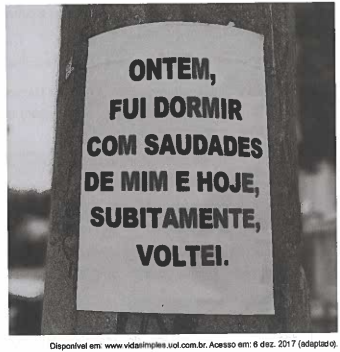
\includegraphics[width=\columnwidth]{subareas/linguagens/image1.png}

Considerando-se a função que os cartazes colados em postes normalmente exercem nas ruas das cidades grandes, esse texto evidencia a
\begin{alternativas}
  \item disseminação da arte poética em um veículo não convencional.
  \item manutenção da expectativa das pessoas ao andarem pelas ruas.
  \item necessidade de exposição de poemas pequenos em diferentes suportes.
  \item característica corriqueira do suporte lambe-lambe, muito comum nas ruas.
  \item exposição da beleza escondida das esquinas da cidade de Belo Horizonte.
\end{alternativas}

\label{last-linguagens}

%%% Local Variables:
%%% mode: latex
%%% TeX-master: "../main"
%%% End:

\noindent{\small\textbf{CIÊNCIAS HUMANAS E SUAS TECNOLOGIAS}}

\noindent\textbf{Questões 01 a 40} %arrumar o número


%
% História - Felipe
%

\questao %(Enem 2018)
\citacao{
A rebelião luso-brasileira em Pernambuco começou a ser urdida em 1644 e explodiu em 13 de junho de 1645, dia de Santo Antônio. Uma das primeiras medidas de João Fernandes foi decretar nulas as dívidas que os rebeldes tinham com os holandeses. Houve grande adesão da “nobreza da terra”, entusiasmada com esta proclamação heroica.}{
VAINFAS, R. Guerra declarada e paz fingida na restauração portuguesa. Tempo, n. 27, 2009.
}
O desencadeamento dessa revolta na América portuguesa seiscentista foi o resultado do(a)
\begin{alternativas}
\item fraqueza bélica dos protestantes batavos.
\item comércio transatlântico da África ocidental.
\item auxílio financeiro dos negociantes flamengos.
\item diplomacia internacional dos Estados ibéricos.
\item interesse econômico dos senhores de engenho.
\end{alternativas}

\questao %Enem 2016
\citacao{
A regulação das relações de trabalho compõe uma estrutura complexa, em que cada elemento se ajusta aos demais. A Justiça do Trabalho é apenas uma das peças dessa vasta engrenagem. A presença de representantes classistas na composição dos órgãos da Justiça do Trabalho é também resultante da montagem dessa regulação. O poder normativo também reflete essa característica. Instituída pela Constituição de 1934, a Justiça do Trabalho só vicejou no ambiente político do Estado Novo instaurado em 1937. }{
ROMITA, A. S. Justiça do Trabalho: produto do Estado Novo. In: PANDOLFI, D. (org.). Repensando o Estado Novo. Rio de Janeiro: FGV, 1999. }
A criação da referida instituição estatal na conjuntura histórica abordada teve por objetivo:
\begin{alternativas}
\item Legitimar os protestos fabris.
\item Ordenar os conflitos laborais. 
\item Oficializar os sindicatos plurais.
\item Assegurar os princípios liberais.
\item Unificar os salários profissionais.
\end{alternativas}

\questao %Enem 2014
\citacao{
A transferência da corte trouxe para a América portuguesa a família real e o governo da Metrópole. Trouxe também, e sobretudo, boa parte do aparato administrativo português. Personalidades diversas e funcionários régios continuaram embarcando para o Brasil atrás da corte, dos seus empregos e dos seus parentes após o ano de 1808. }{
NOVAIS, F. A.; ALENCASTRO, L. F. (Org.). História da vida privada no Brasil. São Paulo: Cia. das Letras, 1997. }
Os fatos apresentados se relacionam ao processo de independência da América portuguesa por terem 
\begin{alternativas}
\item incentivado o clamor popular por liberdade. 
\item enfraquecido o pacto de dominação metropolitana. 
\item motivado as revoltas escravas contra a elite colonial.
\item obtido o apoio do grupo constitucionalista português.
\item provocado os movimentos separatistas das províncias.
\end{alternativas}

\questao %Enem 2014
\citacao{
O problema central a ser resolvido pelo Novo Regime era a organização de outro pacto de poder que pudesse substituir o arranjo imperial com grau suficiente de estabilidade. O próprio presidente Campos Sales resumiu claramente seu objetivo: ``É de lá, dos estados, que se governa a República, por cima das multidões que tumultuam agitadas nas ruas da capital da União. A política dos estados é a política nacional''. }{
CARVALHO, J. M. Os Bestializados: o Rio de Janeiro e a República que não foi. São Paulo: Companhia das Letras, 1987 (adaptado).}
Nessa citação, o presidente do Brasil no período expressa uma estratégia política no sentido de
\begin{alternativas}
\item governar com a adesão popular.
\item ampliar a influência da capital no cenário nacional.
\item conferir maior autonomia às prefeituras.
\item democratizar o poder do governo central.
\item atrair o apoio das oligarquias regionais.
\end{alternativas}

\questao %Enem 2012
De acordo com um estudo recente, na Bahia, entre 1680 e 1797, de 160 filhas nascidas em 53 famílias de destaque, mais de 77\% foram enviadas a conventos, 5\% permaneceram solteiras e apenas 14 se casaram. Tendo em vista que, no período colonial, mesmo entre pessoas livres, a população masculina era maior que a feminina, esses dados sugerem que...
\begin{alternativas}
\item os senhores-de-engenho não deixavam suas filhas casarem com pessoas de nível social e econômico inferior. 
\item entre as mulheres ricas, a devoção religiosa era mais intensa e fervorosa do que entre as mulheres pobres. 
\item os homens brancos preferiam manter sua liberdade sexual a se submeterem ao despotismo dos senhores-de-engenho.
\item a vida na colônia era tão insuportável para as mulheres que elas preferiam vestir o hábito de freiras na Metrópole.
\item a sociedade colonial se pautava por padrões morais que privilegiavam o sexo e a beleza e não o status e a riqueza.
\end{alternativas}

\questao %Enem 2006
A moderna democracia brasileira foi construída entre saltos e sobressaltos. Em 1954, a crise culminou no suicídio do presidente Vargas. No ano seguinte, outra crise quase impediu a posse do presidente eleito, Juscelino Kubitschek. Em 1961, o Brasil quase chegou à guerra civil depois da inesperada renuncia do presidente Jânio Quadros. Três anos mais tarde, um golpe militar depôs o presidente João Goulart, e o país viveu durante vinte anos em regime autoritário. A partir dessas informações, relativas à historia republicana brasileira, assinale a opção correta:
\begin{alternativas}
\item Ao término do governo João Goulart, Juscelino Kubitschek foi eleito presidente da Republica. 
\item A renúncia de Jânio Quadros representou a primeira grande crise do regime republicano brasileiro. 
\item Apos duas décadas de governos militares, Getúlio Vargas foi eleito presidente em eleições diretas.
\item A trágica morte de Vargas determinou o fim da carreira política de João Goulart.
\item No período republicano citado, sucessivamente, um presidente morreu, um teve sua posse contestada, um renunciou e outro foi deposto.
\end{alternativas}

\questao %Enem 2004
Constituição de 1824: ``Art. 98. O Poder Moderador é a chave de toda a organização política, e é delegado privativamente ao Imperador (…) para que incessantemente vele sobre a manutenção da Independência, equilíbrio, e harmonia dos demais poderes políticos (...) dissolvendo a Câmara dos Deputados nos casos em que o exigir a salvação do Estado.'' 
Frei Caneca: ``O Poder Moderador da nova invenção maquiavélica é a chave mestra da opressão da nação brasileira e o garrote mais forte da liberdade dos povos. Por ele, o imperador pode dissolver a Câmara dos Deputados, que é a representante do povo, ficando sempre no gozo de seus direitos o Senado, que é o representante dos apaniguados do imperador.'' (Voto sobre o juramento do projeto de Constituição)\\
Para Frei Caneca, o Poder Moderador definido pela Constituição outorgada pelo Imperador em 1824 era
\begin{alternativas}
\item adequado ao funcionamento de uma monarquia constitucional, pois os senadores eram escolhidos pelo Imperador. 
\item eficaz e responsável pela liberdade dos povos, porque garantia a representação da sociedade nas duas esferas do poder legislativo. 
\item arbitrário, porque permitia ao Imperador dissolver a Câmara dos Deputados, o poder representativo da sociedade.
\item neutro e fraco, especialmente nos momentos de crise, pois era incapaz de controlar os deputados representantes da Nação.
\item capaz de responder às exigências políticas da nação, pois supria as deficiências da representação política.
\end{alternativas}

\questao %Enem 2020
\citacao{
Com efeito, até a destruição de Cartago, o povo e o Senado romano governavam a República em harmonia e sem paixão, e não havia entre os cidadãos luta por glória ou dominação; o medo do inimigo mantinha a cidade no cumprimento do dever. Mas, assim que o medo desapareceu dos espíritos, introduziram-se os males pelos quais a prosperidade tem predileção, isto é, a libertinagem e o orgulho.}{
SALÚSTIO. \textit{A conjuração de Catilina/A guerra de Jugurta.} Petrópolis: Vozes, 1990 (adaptado).}
O acontecimento histórico mencionado no texto de Salústio, datado de I a.C., manteve correspondência com o processo de 
\begin{alternativas}
\item demarcação de terras públicas.   
\item imposição da escravidão por dividas.   
\item restrição da cidadania por parentesco.   
\item restauração de instituições ancestrais.   
\item expansão das fronteiras extrapeninsulares. 
\end{alternativas}

\questao %Enem 2018
\citacao{
Temos vivido, como nação, atormentados pelos males modernos e pelos males do passado, pelo velho e pelo novo, sem termos podido conhecer uma história de rupturas revolucionárias. Não que não tenhamos nos modernizado e chegado ao desenvolvimento. Mas não eliminamos relações, estruturas e procedimentos contrários ao espírito do tempo. Nossa modernização tem sido conservadora.}{
NOGUEIRA, M. \textit{As possibilidades da política: ideias para a reforma democrática do Estado.} Rio de Janeiro: Paz e Terra, 1998.}
O texto apresenta uma análise recorrente sobre o processo de modernização do Brasil na segunda metade do século XX. De acordo com a análise, uma característica desse processo reside na(s)
\begin{alternativas}
\item uniformização técnica dos espaços de produção.    
\item construção municipalista do regime representativo.    
\item organização estadual das agremiações partidárias.    
\item limitações políticas no estabelecimento de reformas sociais.    
\item restrições financeiras no encaminhamento das demandas ruralistas. 
\end{alternativas}

\questao %Enem 2018
\citacao{Torna-se importante, portanto, salientar que as pautas econômicas dominantes não se incompatibilizavam com demandas políticas ou por garantia de direitos contra as decisões da própria Justiça do Trabalho. Pelo contrário, muitas greves incluíam várias demandas de natureza distinta, e mesmo em demandas primariamente econômicas, colocava-se muitas vezes a dimensão do enfrentamento político. Em todos esses casos, confirma-se a hipótese de que direitos instituídos ou garantias das convenções coletivas, respaldadas pela Justiça do Trabalho, não significavam conquistas materiais às quais os trabalhadores tivessem acesso líquido e certo. Era preciso muitas vezes recorrer às greves para garantir direitos conquistados.}{
MATTOS, M. B. Greves, sindicatos e repressão policial no Rio de Janeiro (1954-1964). \textit{Revista Brasileira de História}, n. 47, 2004 (adaptado).}
De acordo com o texto, um dos problemas com os quais as organizações sindicais de trabalhadores se defrontavam, de 1954 a 1964, era o descompasso entre
\begin{alternativas}
\item legislação e realidade social.    
\item profissão e formação técnica.    
\item meio rural e cidades industriais.    
\item população e representação parlamentar.    
\item empresariado nacional e capitais estrangeiros.
\end{alternativas}

%
% Geografia - Luis Felipe
%

\questao
O gráfico abaixo representa a relação entre o tamanho e a totalidade dos imóveis rurais no Brasil. Que característica da estrutura fundiária brasileira está evidenciada no gráfico apresentado?
\citacao{
\begin{center}
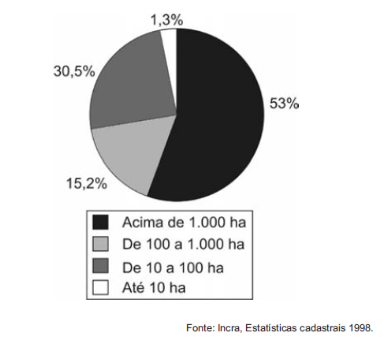
\includegraphics[trim= 0 45 55 0, clip, width=.8\columnwidth]{subareas/ciencias_humanas/geografia-1.png}
\end{center}
}{Fonte: Incra, Estatísticas cadastrais 1998.}
\begin{alternativas}
\item A concentração de terras nas mãos de poucos.
\item A existência de poucas terras agricultáveis.
\item O domínio territorial dos minifúndios.
\item A primazia da agricultura familiar.
\item A debilidade dos plantations modernos.
\end{alternativas}

\questao
\citacao{
\textbf{TEXTO I} – A nossa luta é pela democratização da propriedade da terra, cada vez mais concentrada em nosso país. Cerca de 1\% de todos os proprietários controla 46\% das terras. Fazemos pressão por meio da ocupação de latifúndios improdutivos e grandes propriedades, que não cumprem a função social, como determina a Constituição de 1988. Também ocupamos as fazendas que têm origem na grilagem de terras públicas.}{
Disponível em www.mst.org.br – acessado em 25 de agosto de 2011 (adaptado).}
\citacao{
\textbf{TEXTO II} – O pequeno proprietário rural é igual a um pequeno proprietário de loja: quanto menor o negócio, mais difícil de manter, pois tem que ser produtivo e os encargos são difíceis de custear. Sou a favor de propriedades produtivas e sustentáveis, que gerem empregos. Apoiar uma empresa produtiva que gere emprego é muito mais barato e gera muito mais do que apoiar a reforma agrária.}{
LESSA, C. Disponível em www.observatoriopolitico.org.br, acessado em 25 de agosto de 2011 (adaptado).}
Nos fragmentos dos textos, os posicionamentos em relação à reforma agrária se opõem. Isso acontece porque os autores associam a reforma agrária, respectivamente, à
\begin{alternativas}
\item Redução do inchaço urbano e à crítica ao minifúndio camponês.
\item Ampliação da renda nacional e à prioridade ao mercado externo.
\item Contestação da mecanização agrícola e ao combate ao êxodo rural.
\item Privatização de empresas estatais e ao estímulo ao crescimento econômico.
\item Correção de distorções históricas e ao prejuízo ao agronegócio.
\end{alternativas}

\questao
A dinâmica de transformação das cidades tende a apresentar como consequência a expansão das áreas periféricas pelo(a)
\begin{alternativas}
\item Direcionamento organizado do fluxo de pessoas, devido à existência de um grande número de serviços.
\item Delimitação de áreas para uma ocupação organizada do espaço físico, melhorando a qualidade de vida.
\item Crescimento descontrolado da população urbana e aumento da especulação imobiliária.
\item Implantação de políticas públicas que promovem a moradia e o direito à cidade aos seus moradores.
\item Reurbanização de moradias nas áreas centrais, mantendo o trabalhador próximo ao seu emprego, diminuindo os deslocamentos para a periferia.
\end{alternativas}

\questao
\citacao{
Subindo morros, margeando córregos ou penduradas em palafitas, as favelas fazem parte da paisagem de um terço dos municípios do país, abrigando mais de 10 milhões de pessoas, segundo dados do Instituto Brasileiro de Geografia e Estatística (IBGE).}{
MARTINS A. R. \textit{A favela como um espaço da cidade.}\\
Disponível em http://www.revistaescola.abril.com.br Acessado em 31 de julho de 2010. }
A situação das favelas no país reporta a graves problemas de desordenamento territorial. Nesse sentido, uma característica comum a esses espaços tem sido
\begin{alternativas}
\item O planejamento para a implantação de infraestruturas urbanas necessárias para atender às necessidades básicas dos moradores.
\item A organização de associações de moradores interessadas na melhoria do espaço urbano e financiadas pelo poder público.
\item A presença de ações referentes à educação ambiental com consequente preservação dos espaços naturais circundantes.
\item A ocupação de áreas de risco suscetíveis a enchentes ou desmoronamentos com consequentes perdas materiais e humanas.
\item O isolamento socioeconômico dos moradores ocupantes desses espaços com a resultante multiplicação de políticas que tentam reverter esse quadro.
\end{alternativas}

\questao
Leia a descrição de quatro grandes tipos climáticos do Brasil e, em seguida, examine o mapa, que representa a divisão regional do país em grandes tipos climáticos.\\
1. Chuvas escassas e irregulares, com precipitações médias de 500 a 700 mm, e temperaturas elevadas, com médias de 28 °C.\\
2. Chuvas entre 2 000 e 3 000 mm e elevadas temperaturas durante todo o ano, com médias de 26 °C.\\
3. Regular distribuição das chuvas durante o ano e temperaturas mais amenas, com médias inferiores a 18 °C e esporádica queda de neve.\\
4. Duas estações bem marcantes: uma chuvosa e quente, com 1 200 mm de precipitação e médias térmicas de 24 °C, e outra seca e fria, com 200 mm de chuvas e 17 °C de média térmica.\\
\citacao{
\begin{center}
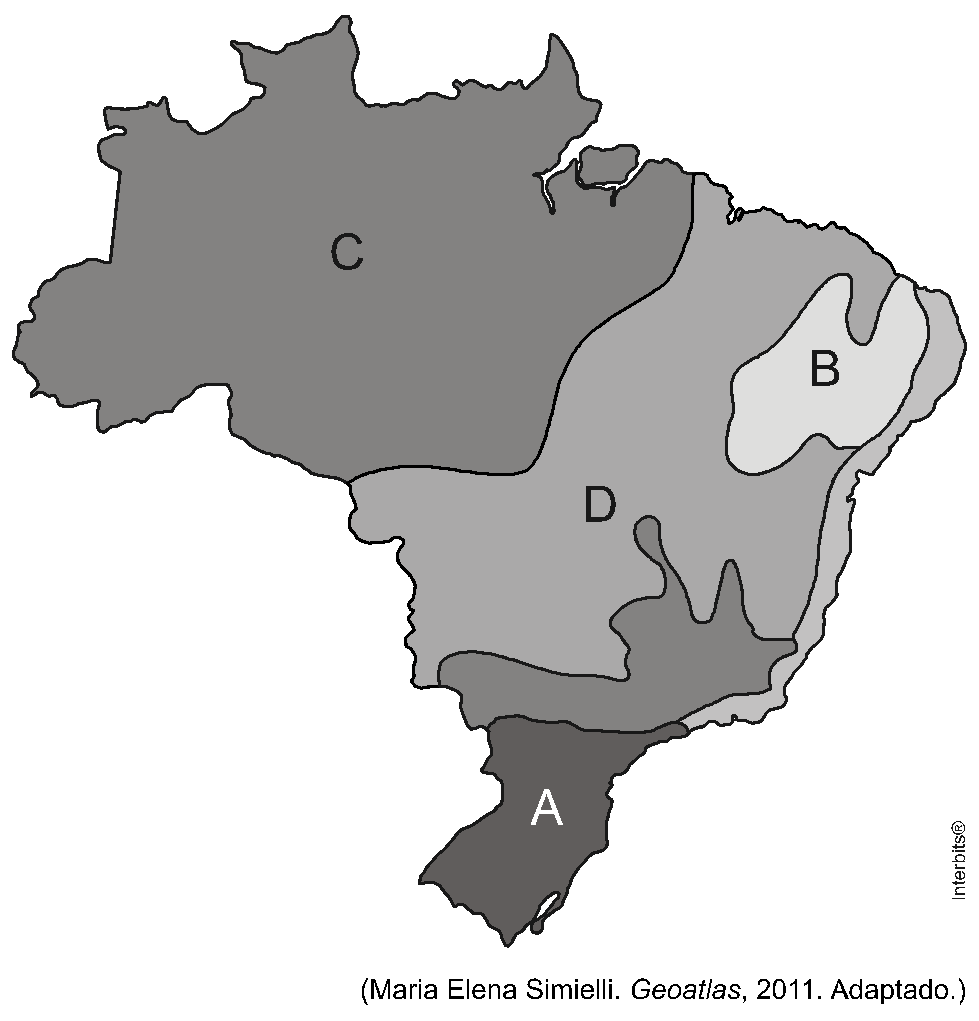
\includegraphics[trim= 0 45 0 0,
clip,width=\columnwidth]{subareas/ciencias_humanas/geografia-2.png}
\end{center}
}{
(Maria Elena Smielli. \textit{Geoatlas}, 2011. Adaptado)}
Assinale a alternativa que contém a correta associação entre a descrição climática e sua área de ocorrência.
\begin{alternativas}
\item 1B; 2C; 3A; 4D.   
\item 1C; 2A; 3B; 4D.   
\item 1B; 2A; 3D; 4C.   
\item 1A; 2C ; 3D; 4B.
\item 1C; 2B; 3D; 4A.
\end{alternativas}

\questao
Assinale a alternativa que indica corretamente as zonas climáticas indicadas abaixo:\\
I. Verões quentes e secos; vegetação com oliveiras e parreiras.\\
II. Quatro estações bem definidas; solos escuros e férteis; vegetação aciculifoliada.\\
III. Clima quente e úmido; solos expostos a laterização; vegetação densa e hidrófila.
\begin{alternativas}
\item I – Tropical; II – Polar; III – Equatorial.
\item I – Mediterrânea; II – Tropical; III – Equatorial.
\item I – Temperada; II – Semiárida; III – Polar.
\item I – Mediterrânea; II – Temperada; III – Tropical.
\item I – Equatorial;  II – Temperada; III – Tropical.
\end{alternativas}

\questao
{\itshape O fenômeno dos ``rios voadores''\\
``Rios voadores'' são cursos de água atmosféricos, invisíveis, que passam por cima de nossas cabeças transportando umidade e vapor de água da bacia Amazônica para outras regiões do Brasil. A floresta Amazônica funciona como uma bomba d’água. Ela ``puxa'' para dentro do continente umidade evaporada do oceano Atlântico que, ao seguir terra adentro, cai como chuva sobre a floresta. Pela ação da evapotranspiração da floresta, as árvores e o solo devolvem a água da chuva para a atmosfera na forma de vapor de água, que volta a cair novamente como chuva mais adiante. O Projeto Rios Voadores busca entender mais sobre a evapotranspiração da floresta Amazônica e a importante contribuição da umidade gerada por ela no regime de chuvas do Brasil.}\\
A partir da leitura do texto e da observação do mapa, é correto afirmar que, no Brasil,
\begin{alternativas}
\item cada vez mais, a floresta é substituída por agricultura ou pastagem, procedimento que promove o desenvolvimento econômico, sem influenciar, significativamente, o clima na América do Sul.   
\item a destruição da Amazônia, sobretudo pela expansão da pecuária e do cultivo de soja, pode alterar consideravelmente a produção de umidade e as chuvas na América do Sul, especialmente no sudeste brasileiro.
\item o atual desenvolvimento da Amazônia não afeta o sistema hidrológico, devido à aplicação de medidas rigorosas contra o desmatamento e danos à biodiversidade da floresta.   
\item os mecanismos climatológicos devem ser considerados na avaliação dos riscos decorrentes de ações como o desmatamento, as queimadas, a abertura de novas fronteiras agrícolas e a liberação dos gases do efeito estufa.   
\item a circulação atmosférica é dominada por massas de ar carregadas de umidade que, encontrando a barreira natural formada pelos Andes, precipitam-se na encosta leste, alimentando as bacias hidrográficas do país.
\end{alternativas}

\questao
\citacao{
{\itshape ``A chegada dos colonizadores, invadindo e ocupando o nosso continente – até aí chamado Aby ayala pelas populações indígenas -, representava a chegada de um novo modelo civilizatório, com o despojo das riquezas naturais dos nossos países, da destruição das populações indígenas e a introdução da pior das selvagerias: a escravidão. Chegaram com a espada e a cruz, para dominar e oprimir, para impor seu poder militar e tentar impor sua religião. (...) Durante mais de 4 séculos fomos reduzidos a isso. Os ciclos econômicos da nossa história foram determinados não por decisões das populações locais, mas das necessidades e interesses do mercado mundial, controlado pelas potências colonizadoras. Pau brasil, açúcar, café e borracha no nosso caso. Ouro, prata, cobre, carne, couro, e outras tantas riquezas do novo continente, foram sendo reiteradamente dilapidados em favor do enriquecimento das potências colonizadoras europeias.''}}{
– Emir Sader, Portal VioMundo (13/10/2011)}
Seguindo a lógica proposta pelo autor do fragmento apresentado, o desenvolvimento econômico do Brasil:
\begin{alternativas}
\item Foi autônomo, atendendo às demandas econômicas e sociais nacionais desde a época da colonização.
\item Já superou a influência histórica do domínio europeu, a exemplo do racismo e da exploração econômica, extintos.
\item Sempre atendeu às demandas impostas pelos interesses hegemônicos: primeiro da Europa, depois dos EUA e hoje, também, da China.
\item Foi influenciado pela colonização europeia apenas do ponto de vista econômico, uma vez que o desenvolvimento social contou somente com influências locais.
\item Só não foi bem sucedido pela insistente presença do Estado, que negou a autonomia do Brasil ao priorizar as políticas sociais ao invés dos investimentos econômicos.
\end{alternativas}

\questao
Sobre a globalização dos problemas ambientais é correto afirmar:\\
I - Após a Revolução Industrial, a Natureza passou a ser vista como uma fonte de recursos econômicos a ser explorada por meio de instrumentos cada vez mais sofisticados, criados pela ciência e pela tecnologia. Nesse processo, o meio ambiente foi submetido a uma contínua devastação, pondo em risco o equilíbrio do planeta e afetando a vida de toda a humanidade.\\
II - Nas últimas décadas do século XX, com o agravamento dos problemas ambientais, a sociedade se mobilizou para tentar deter os efeitos nocivos das atividades econômicas, predatórias e poluentes, porém os interesses financeiros continuam a se sobrepor à consciência ambiental.\\
III - Grupos ecológicos se multiplicaram e a pressão social resultou na aprovação pelos poderes públicos de leis de proteção ao meio ambiente, apesar de serem muitas vezes desrespeitadas.\\
IV - No âmbito internacional, a preservação do meio ambiente passou a constituir elemento importante de um país para negociar a comercialização de seus produtos e recebimento de empréstimos.\\
Estão corretas apenas as afirmações:
\begin{alternativas}
\item I e II.
\item II e III.
\item III e IV
\item I, III e IV.
\item I, II, III e IV.
\end{alternativas}

\questao
Ao analisar o avanço tecnológico ocorrido durante o processo de Globalização é correto afirmar:
\begin{alternativas}
\item Os avanços tecnológicos aconteceram de maneira simultânea em todo o planeta.
\item O setor de serviço perdeu espaço no mundo globalizado, enquanto a indústria “verde” ganhou terreno devido à pressão do movimento ecologista.
\item Observa-se uma tendência dos monopólios dos meios de comunicação asiáticos em detrimento das empresas americanas que dominavam o mercado.
\item O crescimento econômico dos países em desenvolvimento tornou-se uma realidade, pois agora o saber é difundido democraticamente através da internet.
\item Os fluxos de informações e capitais estão em crescente aumento, obedecendo a nova tendência tecnológica de um capitalismo informacional.
\end{alternativas}

%
% Sociologia Marina
%

\questao %Enem 2020
\citacao{
A propriedade compreende, em seu conteúdo e alcance, além do tradicional direito de uso, gozo e disposição por parte de seu titular, a obrigatoriedade do atendimento de sua função social, cuja definição é inseparável do requisito obrigatório do uso racional da propriedade e dos recursos ambientais que lhe são integrantes. O proprietário, como membro integrante da comunidade, se sujeita a obrigações crescentes que, ultrapassando os limites do direito de vizinhança, no âmbito do direito privado, abrangem o campo dos direitos da coletividade, visando o bem-estar geral, no âmbito do direito público.}{
JELINEK. R O princípio da função social da propriedade é sua repercussão sobre o sistema do Código Civil. Disponível em: www.mp.rs.gov.br. Acesso em 20 fev. 2013}
Os movimentos em prol da reforma agrária, que atuam com base no conceito de direito à
propriedade apresentado no texto, propõem-se a
\begin{alternativas}
\item Reverter o processo de privatização fundiária.
\item Ressaltar a inviabilidade da produção latifundiária.
\item Defender a desapropriação dos espaços improdutivos.
\item Impedir a produção exportadora nas terras agricultáveis.
\item Coibir o funcionamento de empresas agroindustriais no campo.
\end{alternativas}

\questao %Enem 2017
\citacao{
No Brasil, assim como em vários outros países, os modernos movimentos LGBT representam um desafio às formas de condenação e perseguição social contra desejos e comportamentos sexuais anticonvencionais associados à vergonha, imoralidade, pecado, degeneração, doença. Falar do movimento LGBT implica, portanto, chamar a atenção para a sexualidade como fonte de estigmas, intolerância, opressão.
}{
SIMÕES, J. Homossexualidade e movimento LGBT: estigma, diversidade e cidadania. In: BOTELHO, A.; SCHWARCZ, L. M. Cidadania, um projeto em construção. São Paulo: Claro Enigma, 2012 (adaptado).}
O movimento social abordado justifica-se pela defesa do direito de
\begin{alternativas}
\item Organização sindical.
\item Participação partidária.
\item Manifestação religiosa.
\item Formação profissional.
\item Afirmação identitária.
\end{alternativas}

\questao %Enem 2015
\citacao{
Ninguém nasce mulher: torna-se mulher. Nenhum destino biológico, psíquico, econômico define a forma que a fêmea humana assume no seio da sociedade; é o conjunto da civilização que elabora esse produto intermediário entre o macho e o castrado que qualificam o feminino.}{
BEAUVOIR, S. O segundo sexo. Rio de Janeiro: Nova Fronteira, 1980.}
Na década de 1960, a proposição de Simone de Beauvoir contribuiu para estruturar um movimento social que teve como marca o(a)
\begin{alternativas}
\item Ação do Poder Judiciário para criminalizar a violência sexual.
\item Pressão do Poder Legislativo para impedir a dupla jornada de trabalho.
\item Organização de protestos públicos para garantir a igualdade de gênero.
\item Oposição de grupos religiosos para impedir os casamentos homoafetivos.
\item Estabelecimento de políticas governamentais para promover ações afirmativas.
\end{alternativas}

\questao %Enem 2020 - Digital
\citacao{
A masculinidade, assim como a feminilidade, é uma construção histórica e cultural. Em nossa cultura, a dança caracteriza-se, no sentido geral, como um universo predominantemente feminino. Homens que dançam são geralmente considerados homossexuais, por não se enquadrarem dentro das normas culturais hegemônicas de gênero e sexualidade. Por outro lado, demonstram a não existência de um único tipo de masculinidade, enfatizando que as identidades humanas são múltiplas e plurais. No contexto da dança, as representações hegemônicas de gênero e as regulações sociais que essas impõem não se manifestam deforma igual em todas as modalidades de dança. Persiste essa forte representação cultural ocidental que associa o balé à feminilidade e à homossexualidade. Em outras danças, ela não se revela tão forte, e os homens não aparecem em menor número, como nas tradicionais danças folclóricas ou no moderno hip hop.}{
ANDREOLI, G. S. Representações de masculinidade na dança contemporânea. Movimento, n. 1, 2011 (adaptado).}
\begin{alternativas}
\item padronização da inserção dos homens nessas manifestações corporais.
\item identificação de como essas práticas regulam uma única masculinidade.
\item reconhecimento das diferentes masculinidades.
\item contestação das normas sociais pelo balé.
\item reforço de uma feminilidade hegemônica.
\end{alternativas}

\questao
\textbf{TEXTO I}
\citacao{
\begin{center}
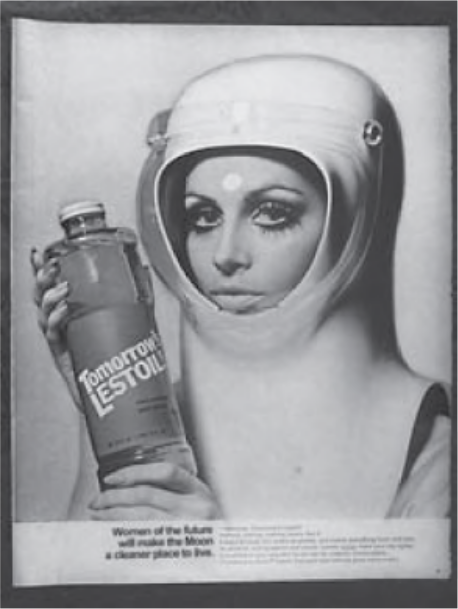
\includegraphics[width=\columnwidth]{subareas/ciencias_humanas/sociologia-1.png}
\textbf{Tradução: ``As mulheres do futuro farão da Lua um lugar mais limpo para se viver''}
\end{center}
}{
Disponível em: www.propagandashistoricas.com.br. Acesso em: 16 out. 2015.}
\textbf{TEXTO II}
\citacao{
\begin{center}
\textbf{Metade da nova equipe da Nasa é composta por mulheres} 
\end{center}
Até hoje, cerca de 350 astronautas americanos já estiveram no espaço, enquanto as mulheres não chegam a ser um terço desse número. Após o anúncio da turma composta 50\% por mulheres, alguns internautas escreveram comentários machistas e desrespeitosos sobre a escolha nas redes sociais.}{
Disponível em: https://catracalivre.com.br. Acesso em: 10 mar. 2016}
A comparação entre o anúncio publicitário de 1968 e a repercussão da notícia de 2016 mostra a:
\begin{alternativas}
\item elitização da carreira científica.
\item qualificação da atividade doméstica.
\item ambição de indústrias patrocinadoras.
\item manutenção de estereótipos de gênero.
\item equiparação de papéis nas relações familiares.
\end{alternativas}

\questao %Enem 2014
\citacao{
O cidadão norte-americano desperta num leito construído segundo padrão originário do Oriente Próximo, mas modificado na Europa Setentrional antes de ser transmitido à América. Sai debaixo de cobertas feitas de algodão cuja planta se tornou doméstica na Índia. No restaurante, toda uma série de elementos tomada de empréstimo o espera. O prato é feito de uma espécie de cerâmica inventada na China. A faca é de aço, liga feita pela primeira vez na Índia do Sul; o garfo é inventado na Itália medieval; a colher vem de um original romano. Lê notícias do dia impressas em caracteres inventados pelos antigos semitas, em material inventado na China e por um processo inventado na Alemanha.}{
LINTON, R. \textit{O homem: uma introdução à antropologia.} São Paulo: Martins, 1959 (adaptado)}
A situação descrita é um exemplo de como os costumes resultam da:
\begin{alternativas}
\item assimilação de valores de povos exóticos.
\item experimentação de hábitos sociais variados.
\item recuperação de heranças da Antiguidade Clássica.
\item fusão de elementos de tradições culturais diferentes.
\item valorização de comportamento de grupos privilegiados.
\end{alternativas}

\questao %Enem 2011
\citacao{
A Lei 10.639, de 9 de janeiro de 2003, inclui no currículo dos estabelecimentos de ensino fundamental e médio, oficiais e particulares, a obrigatoriedade do ensino sobre História e Cultura Afro-Brasileira e determina que o conteúdo programático incluirá o estudo da História da África e dos africanos, a luta dos negros no Brasil, a cultura negra brasileira e o negro na formação da sociedade nacional, resgatando a contribuição do povo negro nas áreas social, econômica e política pertinentes à História do Brasil, além de instituir, no calendário escolar, o dia 20 de novembro como data comemorativa do ``Dia da Consciência Negra''.}{
Disponível em: http://www.planalto.gov.br. Acesso em: 27 jul. 2010
(adaptado).}
A referida lei representa um avanço não só para a educação nacional, mas também para a sociedade brasileira, porque
\begin{alternativas}
\item Legitima o ensino das ciências humanas nas escolas.
\item Divulga conhecimentos para a população afro-brasileira.
\item Reforça a concepção etnocêntrica sobre a África e sua cultura.
\item Garante aos afrodescendentes a igualdade no acesso à educação.
\item Impulsiona o reconhecimento da pluralidade étnicoracial do país.
\end{alternativas}

\questao %Enem 2018
\citacao{
Num país que conviveu com o trabalho escravo durante quatro séculos, o trabalho doméstico é ainda considerado um subemprego. E os indivíduos que atuam nessa área são, muitas vezes, vistos pelos patrões como um mal necessário: é preciso ter em casa alguém que limpe o banheiro, lave a roupa, tire o pó e arrume a gaveta. Existe uma inegável desvalorização das atividades domésticas em relação a outros tipos de trabalho.}{
RANGEL, C. Domésticas: nascer, deixar, permanecer ou simplesmente estar. In: SOUZA, E. (Org.). \textbf{Negritude, cinema e educação.} Belo Horizonte: Mazza, 2011 (adaptado).}
Objeto de legislação recente, o enfrentamento do problema mencionado resultou na
\begin{alternativas}
\item criação de novos ofícios.
\item ampliação de direitos sociais.
\item redução da desigualdade de gênero.
\item fragilização da representação sindical.
\item erradicação da atividade informal.
\end{alternativas}

\questao %Enem PPL 2016
\textbf{TEXTO I}
\citacao{
\begin{center}
Cidadão\\
Tá vendo aquele edifício, moço?\\
Ajudei a levantar\\
Foi um tempo de aflição\\
Eram quatro condução\\
Duas pra ir, duas pra voltar\\
Hoje depois dele pronto\\
Olho pra cima e fico tonto\\
Mas me vem um cidadão\\
E me diz desconfiado\\
“Tu tá aí admirado\\
Ou tá querendo roubar?”\\
Meu domingo tá perdido\\
Vou pra casa entristecido\\
Dá vontade de beber\\
E pra aumentar meu tédio\\
Eu nem posso olhar pro prédio\\
Que eu ajudei a fazer.\\
\end{center}}{
BARBOSA. L. In: ZÉ RAMALHO, 20 Super Sucessos. Rio de Janeiro: Sony Music. 1999 - fragmento}
\textbf{TEXTO II}
\citacao{
O trabalhador fica mais pobre à medida que produz mais riqueza e sua produção cresce em força e extensão. O trabalhador torna-se uma mercadoria ainda mais barata à medida que cria mais bens. Esse fato simplesmente subentende que o objeto produzido pelo trabalho, o seu produto, agora se lhe opõe como um ser estranho, como uma força independente do produtor.}{
MARX, K. Manuscritos econômicos-filosóficos (Os Primeiros). São Paulo: Boitempo Editorial, 2004}
Com base nos textos. a relação entre trabalho e modo de produção capitalista é:
\begin{alternativas}
\item Baseada na desvalorização do trabalho especializado e no aumento da demanda social por novos postos de emprego.
\item Fundada no crescimento proporcional entre o número de trabalhadores e o aumento da produção de bens e serviços.
\item Estruturada na distribuição equânime de renda e no declínio do capitalismo industrial e tecnocrata.
\item Instaurada a partir do fortalecimento da luta de classes e da criação da economia solidária.
\item Derivada do aumento da riqueza e da ampliação da exploração do trabalhador.
\end{alternativas}

\questao %Enem PPL 2013
\citacao{
O servo pertence à terra e rende frutos ao dono da terra. O operário urbano livre, ao contrário, vende-se a si mesmo e, além disso, por partes. Vende em leilão 8,10,12,15 horas da sua vida, dia após dia, a quem melhor pagar, ao proprietário das matérias-primas, dos instrumentos de trabalho e dos meios de subsistência, isto é, ao capitalista.}{
MARX, K. Trabalho assalariado e capital \& salário, preço e lucro. São Paulo: Expressão
Popular, 2010}
O texto indica que houve uma transformação dos espaços urbanos e rurais com a implementação do sistema capitalista, devido às mudanças tecnossociais ligadas ao:
\begin{alternativas}
\item Desenvolvimento agrário e ao regime de servidão.
\item Aumento da produção rural, que fixou a população nesse meio.
\item Desenvolvimento das zonas urbanas e às novas relações de trabalho.
\item Aumento populacional das cidades associado ao regime de servidão.
\item Desenvolvimento da produção urbana associada às relações servis de trabalho.
\end{alternativas}

%
% Filosofia - Rafael
%

\questao
\citacao{
Alguns dos desejos são naturais e necessários; outros, naturais e não necessários; outros, nem naturais nem necessários, mas nascidos de vã opinião. Os desejos que não nos trazem dor se não satisfeitos não são necessários, mas o seu impulso pode ser facilmente desfeito, quando é difícil obter sua satisfação ou parecem geradores de dano.}{
EPICURO DE SAMOS. ``Doutrinas principais''. In: SANSON, V. F. Textos de filosofia. Rio de Janeiro: Eduff, 1974.}
No fragmento da obra filosófica de Epicuro, o homem tem como fim
\begin{alternativas}
\item defender a indiferença e a impossibilidade de se atingir o saber.
\item valorizar os deveres e as obrigações sociais.
\item alcançar o prazer moderado e a felicidade.
\item aceitar o sofrimento e o rigorismo da vida com resignação.
\end{alternativas}

\questao
\citacao{
Uma norma só deve pretender validez quando todos os que possam ser concernidos por ela cheguem (ou possam chegar), enquanto participantes de um discurso prático, a um acordo quanto à validade dessa norma.}{
HABERMAS, J. Consciência moral e agir comunicativo. Rio de Janeiro: Tempo Brasileiro, 1989.}
Segundo Habermas, a validez de uma norma deve ser estabelecida pelo(a):
\begin{alternativas}
\item técnica científica, que aumenta o poder do homem.
\item razão comunicativa, que requer um consenso.
\item liberdade humana, que consagra a vontade.
\item poder político, que se concentra no sistema partidário.
\item conhecimento filosófico, que expressa a verdade.
\end{alternativas}

\questao
\citacao{
Compreende-se assim o alcance de uma reivindicação que surge desde o nascimento da cidade na Grécia antiga: a redação das leis. Ao escrevê-las, não se faz mais que assegurar-lhes permanência e fixidez. As leis tornam-se bem comum, regra geral, suscetível de ser aplicada a todos da mesma maneira.}{
VERNANT, J. P. As origens do pensamento grego. Rio de Janeiro: Bertrand Brasil, 1992 (adaptado).}
Para o autor, a reivindicação atendida na Grécia antiga, ainda vigente no mundo contemporâneo, buscava garantir o seguinte princípio:
\begin{alternativas}
\item Tripartição — separação entre os poderes políticos estatais.
\item Isonomia — igualdade de tratamento aos cidadãos.
\item Elegibilidade — permissão para candidatura aos cargos públicos.
\item Equiparação — igualdade de gênero na participação política.
\item Transparência — acesso às informações governamentais.
\end{alternativas}

\questao
\citacao{
Hoje, a indústria cultural assumiu a herança civilizatória da democracia de pioneiros e empresários, que tampouco desenvolvera uma fineza de sentido para os desvios espirituais. Todos são livres para dançar e para se divertir, do mesmo modo que, desde a neutralização histórica da religião, são livres para entrar em qualquer uma das inúmeras seitas. Mas a liberdade de escolha de ideologia, que reflete sempre a coerção econômica, revela-se em todos os setores como a liberdade de escolher o que é sempre a mesma coisa.}{
ADORNO, T; HORKHEIMER, M. A dialética do esclarecimento: fragmentos filosóficos. Rio de Janeiro: Zahar, 1995.}
A liberdade de escolha na civilização ocidental, de acordo com a análise do texto, é um(a):
\begin{alternativas}
\item legado social.
\item ilusão da contemporaneidade.
\item produto da moralidade.
\item conquista da humanidade.
\item patrimônio político.
\end{alternativas}

\questao
\citacao{
Sentimos que toda satisfação de nossos desejos advinda do mundo assemelha-se à esmola que mantém hoje o mendigo vivo, porém prolonga amanhã a sua fome. A resignação, ao contrário, assemelha-se à fortuna herdada: livra o herdeiro para sempre de todas as preocupações.}{
SCHOPENHAUER, A. Aforismo para a sabedoria da vida. São Paulo: Martins Fontes, 2005.} O trecho destaca uma ideia remanescente de uma tradição filosófica ocidental, segundo a qual a felicidade se mostra indissociavelmente ligada à
\begin{alternativas}
\item fugacidade do conhecimento empírico.
\item consagração de relacionamentos afetivos.
\item administração da independência interior.
\item liberdade de expressão religiosa.
\item busca de prazeres efêmeros.
\end{alternativas}

\questao
\citacao{
Nunca nos tornaremos matemáticos, por exemplo, embora nossa memória possua todas as demonstrações feitas por outros, se nosso espírito não for capaz de resolver toda espécie de problemas; não nos tornaríamos filósofos, por ter lido todos os raciocínios de Platão e Aristóteles, sem poder formular um juízo sólido sobre o que nos é proposto. Assim, de fato, pareceríamos ter aprendido, não ciências, mas histórias.}{
DESCARTES, R. Regras para a orientação do espírito. São Paulo: Martins Fontes, 1999.}
Em busca pelo saber verdadeiro, o autor considera o conhecimento, de modo crítico, como resultado da
\begin{alternativas}
\item investigação da natureza empírica.
\item retomada da tradição intelectual.
\item imposição de valores ortodoxos.
\item autonomia do sujeito pensante.
\item liberdade do agente moral.
\end{alternativas}

\questao
\textbf{TEXTO I}
\citacao{Fragmento B91: Não se pode banhar duas vezes no mesmo rio, nem substância mortal alcança duas vezes a mesma condição; mas pela intensidade e rapidez da mudança, dispersa e de novo reúne.}{
HERÁCLITO. Fragmentos (Sobre a natureza) São Paulo: Abril Cultural, 1996 (adaptado).}
\textbf{TEXTO II}
\citacao{
Fragmento B8: São muitos os sinais de que o ser é ingênito e indestrutível, pois é compacto, inabalável sem fim; não foi nem será, pois é agora um todo homogêneo, uno, contínuo.}{
PARMÊNIDES. Da natureza. São Paulo: Loyola, 2002 (adaptado).}
Os fragmentos do pensamento pré-socrático expõem uma oposição que se insere no
campo das
\begin{alternativas}
\item investigações do pensamento sistemático.
\item preocupações do período mitológico.
\item discussões de base ontológica.
\item habilidade da retórica sofística.
\item verdades do mundo sensível.
\end{alternativas}

\questao
\citacao{
A arte pré-histórica africana foi incontestavelmente um veículo de mensagens pedagógicas e sociais. Os San, que constituem hoje um povo mais próximo da realidade das representações rupestres, afirmam que seus antepassados lhes explicaram sua visão do mundo a partir desse gigantesco livro que são as galerias. A educação dos povos que desconhecem a escrita está baseada sobretudo na imagem e no som, no audiovisual.}{
KI-ZERBO, J. A arte pré-histórica africana. In: KI-ZERBO, J. (Org.) História geral da África. Brasília: Unesco, 2010.}
De acordo com o texto, a arte mencionada é importante para os povos que a cultivam por colaborar para o(a)
\begin{alternativas}
\item expansão da propriedade individual.
\item surgimento dos laços familiares.
\item rejeição de práticas exógenas.
\item transmissão dos saberes acumulados.
\item ruptura da disciplina hierárquica.
\end{alternativas}

\questao
\citacao{
Montaigne deu o nome para um novo gênero literário; foi dos primeiros a instituir na literatura moderna um espaço privado, o espaço do “eu”, do texto íntimo. Ele cria um novo processo de escrita filosófica, no qual hesitações, autocríticas, correções entram no próprio texto.}{
COELHO, M. Montaigne. São Paulo: Publifolha, 2001 (adaptado).}
O novo gênero de escrita aludido no texto é o(a)
\begin{alternativas}
\item diálogo, que discute assuntos com diferentes interlocutores.
\item carta, que comunica informações para um conhecido.
\item confissão, que relata experiências de transformação.
\item meditação, que propõe preparações para o conhecimento.
\item ensaio, que expõe concepções subjetivas de um tema.
\end{alternativas}

\questao
\citacao{
\begin{center}
Declaração de Salamanca – 1994
\end{center}
Acreditamos e proclamamos que: toda criança tem direito fundamental à educação e deve ser dada a oportunidade de atingir e manter o nível adequado de aprendizagem; toda criança possui características, interesses, habilidades e necessidades de aprendizagem que são únicas; sistemas educacionais deveriam ser designados e programas educacionais deveriam ser implementados no sentido de se levar em conta a vasta diversidade de tais características e necessidades.}{
Disponível em: http://portal.mec.gov.br Acesso em: 4 out. 2015.}
Como signatário da Declaração citada, o Brasil comprometeu-se com a elaboração de políticas públicas educacionais que contemplem a
\begin{alternativas}
\item criação de privilégios.
\item valorização da meritocracia.
\item pluralidade dos sujeitos.
\item contenção dos gastos.
\item padronização do currículo.
\end{alternativas}
\noindent{\small\textbf{CIÊNCIAS DA NATUREZA E SUAS TECNOLOGIAS}}

\noindent\textbf{Questões 61 a 80} %arrumar o número

%
% Biologia - Luan
%

\questao
Nas recentes expedições espaciais que chegaram ao solo de Marte, e através dos sinais fornecidos por diferentes sondas e formas de análise, vem sendo investigada a possibilidade da existência de água naquele planeta. A motivação principal dessas investigações, que ocupam frequentemente o noticiário sobre Marte, deve-se ao fato de que a presença de água indicaria, naquele planeta:
\begin{alternativas}
\item a existência de um solo rico em nutrientes e com potencial para a agricultura. 
\item a existência de ventos, com possibilidade de erosão e formação de canais. 
\item a possibilidade de existir ou ter existido alguma forma de vida semelhante à da Terra. 
\item a possibilidade de extração de água visando ao seu aproveitamento futuro na Terra. 
\item a viabilidade, em futuro próximo, do estabelecimento de colônias humanas em Marte.
\end{alternativas}

\questao
\citacao{
Um molusco, que vive no litoral oeste dos EUA, pode redefinir tudo o que se sabe sobre a divisão entre animais e vegetais. Isso porque o molusco (\textit{Elysia chlorotica}) é um híbrido de bicho com planta. Cientistas americanos descobriram que o molusco conseguiu incorporar um gene das algas e, por isso, desenvolveu a capacidade de fazer fotossíntese. É o primeiro animal a se “alimentar” apenas de luz e CO2, como as plantas.}{
GARATONI, B. Superinteressante. Edição 276, mar. 2010 (adaptado).}
A capacidade de o molusco fazer fotossíntese deve estar associada ao fato de o gene incorporado permitir que ele passe a sintetizar:
\begin{alternativas}
\item clorofila, que utiliza a energia do carbono para produzir glicose. 
\item citocromo, que utiliza a energia da água para formar oxigênio. 
\item clorofila, que doa elétrons para converter gás carbônico em oxigênio. 
\item citocromo, que doa elétrons da energia luminosa para produzir glicose. 
\item clorofila, que transfere a energia da luz para compostos orgânicos.
\end{alternativas}

\questao
Em certos locais, larvas de moscas, criadas em arroz cozido, são utilizadas como iscas para pesca. Alguns criadores, no entanto, acreditam que essas larvas surgem espontaneamente do arroz cozido, tal como preconizado pela teoria da geração espontânea. Essa teoria começou a ser refutada pelos cientistas ainda no século XVII, a partir dos estudos de Redi e Pasteur, que mostraram experimentalmente que:
\begin{alternativas}
\item seres vivos podem ser criados em laboratório. 
\item a vida se originou no planeta a partir de microrganismos. 
\item o ser vivo é oriundo da reprodução de outro ser vivo preexistente. 
\item seres vermiformes e microrganismos são evolutivamente aparentados. 
\item vermes e microrganismos são gerados pela matéria existente nos cadáveres e nos caldos nutritivos, respectivamente.
\end{alternativas}

\questao
O gráfico abaixo representa a evolução da quantidade de oxigênio na atmosfera no curso dos tempos geológicos. O número 100 sugere a quantidade atual de oxigênio na atmosfera, e os demais valores indicam diferentes porcentagens dessa quantidade.
\begin{center}
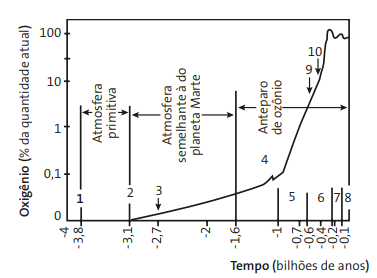
\includegraphics[width=\columnwidth]{subareas/ciencias_natureza/biologia-1.png}
\end{center}
De acordo com o gráfico é correto afirmar que:
\begin{alternativas}
\item as primeiras formas de vida surgiram na ausência de O2. 
\item a atmosfera primitiva apresentava 1\% de teor de oxigênio. 
\item após o início da fotossíntese, o teor de oxigênio na atmosfera mantém-se estável. 
\item desde o Pré-Cambriano, a atmosfera mantém os mesmos níveis de teor de oxigênio. 
\item na escala evolutiva da vida, quando surgiram os anfíbios, o teor de oxigênio atmosférico já se havia estabilizado.
\end{alternativas}

\questao
A partir do primeiro semestre de 2000, a ocorrência de casos humanos de febre amarela silvestre extrapolou as áreas endêmicas, com registro de casos em São Paulo e na Bahia, onde os últimos casos tinham ocorrido em 1953 e 1948. Para controlar a febre amarela silvestre e prevenir o risco de uma reurbanização da doença, foram propostas as seguintes ações: \\
I. Exterminar os animais que servem de reservatório do vírus causador da doença. \\
II. Combater a proliferação do mosquito transmissor. \\
III. Intensificar a vacinação nas áreas onde a febre é endêmica e em suas regiões limítrofes.\\
É efetiva e possível de ser implementada uma estratégia envolvendo a(s) ação(ões): 
\begin{alternativas}
\item II, apenas. 
\item I e II, apenas. 
\item I e III, apenas.
\item II e III, apenas. 
\item I, II e III.
\end{alternativas}

\questao
Na embalagem de um antibiótico, encontra-se uma bula que, entre outras informações, explica a ação do remédio do seguinte modo: ``O medicamento atua por inibição da síntese proteica bacteriana''. Essa afirmação permite concluir que o antibiótico: 
\begin{alternativas}
\item impede a fotossíntese realizada pelas bactérias causadoras da doença e, assim, elas não se alimentam e morrem. 
\item altera as informações genéticas das bactérias causadoras da doença, o que impede a manutenção e a reprodução desses organismos. 
\item dissolve as membranas das bactérias responsáveis pela doença, o que dificulta o transporte de nutrientes e provoca a morte delas.
\item elimina os vírus causadores da doença, pois não conseguem obter as proteínas que seriam produzidas pelas bactérias que parasitam. 
\item interrompe a produção de proteína das bactérias causadoras da doença, o que impede sua multiplicação pelo bloqueio de funções vitais.
\end{alternativas}

\questao
O que têm em comum Noel Rosa, Castro Alves, Franz Kafka, Álvares de Azevedo, José de Alencar e Frédéric Chopin? Todos eles morreram de tuberculose, doença que ao longo dos séculos fez mais de 100 milhões de vítimas. Aparentemente controlada durante algumas décadas, a tuberculose voltou a matar. O principal obstáculo para seu controle é o aumento do número de linhagens de bactérias resistentes aos antibióticos usados para combatê-la. Esse aumento do número de linhagens resistentes se deve a: 
\begin{alternativas}
\item modificações no metabolismo das bactérias, para neutralizar o efeito dos antibióticos e incorporá-los à sua nutrição. 
\item mutações selecionadas pelos antibióticos, que eliminam as bactérias sensíveis a eles, mas permitem que as resistentes se multipliquem. 
\item mutações causadas pelos antibióticos, para que as bactérias se adaptem e transmitam essa adaptação a seus descendentes. 
\item modificações fisiológicas nas bactérias, para torná-las cada vez mais fortes e mais agressivas no desenvolvimento da doença. 
\item modificações na sensibilidade das bactérias, ocorridas depois de passarem um longo tempo sem contato com antibióticos.
\end{alternativas}

\questao
Os anfíbios são animais que apresentam dependência de um ambiente úmido ou aquático. Nos anfíbios, a pele é de fundamental importância para a maioria das atividades vitais, apresenta glândulas de muco para conservar-se úmida, favorecendo as trocas gasosas e, também, pode apresentar glândulas de veneno contra microrganismos e predadores. Segundo a Teoria Evolutiva de Darwin, essas características dos anfíbios representam a:
\begin{alternativas}
\item lei do uso e desuso. 
\item atrofia do pulmão devido ao uso contínuo da pele. 
\item transmissão de caracteres adquiridos aos descendentes. 
\item futura extinção desses organismos, pois estão mal adaptados. 
\item seleção de adaptações em função do meio ambiente em que vivem.
\end{alternativas}

\questao
Fenômenos biológicos podem ocorrer em diferentes escalas de tempo. Assinale a opção que ordena exemplos de fenômenos biológicos, do mais lento para o mais rápido.
\begin{alternativas}
\item germinação de uma semente, crescimento de uma árvore, fossilização de uma samambaia 
\item fossilização de uma samambaia, crescimento de uma árvore, germinação de uma semente 
\item crescimento de uma árvore, germinação de uma semente, fossilização de uma samambaia 
\item fossilização de uma samambaia, germinação de uma semente, crescimento de uma árvore
\item germinação de uma semente, fossilização de uma samambaia, crescimento de uma árvore
\end{alternativas}

\questao
\citacao{
O menor tamanduá do mundo é solitário e tem hábitos noturnos, passa o dia repousando, geralmente em um emaranhado de cipós, com o corpo curvado de tal maneira que forma uma bola. Quando em atividade, se locomove vagarosamente e emite som semelhante a um assobio. A cada gestação, gera um único filhote. A cria é deixada em uma árvore à noite e é amamentada pela mãe até que tenha idade para procurar alimento. As fêmeas adultas têm territórios grandes e o território de um macho inclui o de várias fêmeas, o que significa que ele tem sempre diversas pretendentes à disposição para namorar!}{
Ciência Hoje das Crianças, ano 19, n. 174, nov. 2006 (adaptado).}
Essa descrição sobre o tamanduá diz respeito ao seu:
\begin{alternativas}
\item habitat. 
\item biótopo. 
\item nível trópico. 
\item nicho ecológico. 
\item potencial biótico.
\end{alternativas}

%
% Química - Luan
%

\questao %Enem - MEC
O sol participa do ciclo da água, pois, além de aquecer a superfície da Terra dando origem aos ventos, provoca a evaporação da água dos rios, lagos e mares. O vapor da água, ao se resfriar, condensa em minúsculas gotinhas, que se agrupam formando as nuvens, neblinas ou névoas úmidas. As nuvens podem ser levadas pelos ventos de uma região para outra. Com a condensação e, em seguida, a chuva, a água volta à superfície da Terra, caindo sobre o solo, rios, lagos e mares. Parte dessa água evapora retornando à atmosfera, outra parte escoa superficialmente ou infiltra-se no solo, indo alimentar rios e lagos. Esse processo é chamado de ciclo da água.\\
Considere, então, as seguintes afirmativas:\\
I. A evaporação é maior nos continentes, uma vez que o aquecimento ali é maior do que nos oceanos.\\
II. A vegetação participa do ciclo hidrológico por meio da transpiração.\\
III. O ciclo hidrológico condiciona processos que ocorrem na litosfera, na atmosfera e na biosfera.\\
IV. A energia gravitacional movimenta a água dentro do seu ciclo.\\
V. O ciclo hidrológico é passível de sofrer interferência humana, podendo apresentar desequilíbrios.\\
\begin{alternativas}
\item Somente a afirmativa III está correta.
\item Somente as afirmativas III e IV estão corretas.
\item Somente as afirmativas I, II e V estão corretas.
\item Somente as afirmativas II, III, IV e V estão corretas.
\item Todas as afirmativas estão corretas.
\end{alternativas}

\questao
\citacao{
Quando definem moléculas, os livros geralmente apresentam conceitos como: ``a menor parte da substância capaz de guardar suas propriedades''. A partir de definições desse tipo, a ideia transmitida ao estudante é a de que o constituinte isolado (moléculas) contém os atributos do todo. É como dizer que uma molécula de água possui densidade, pressão de vapor, tensão superficial, ponto de fusão, ponto de ebulição etc. Tais propriedades pertencem ao conjunto, isto é, manifestam-se nas relações que as moléculas mantêm entre si.}{
Adaptado de OLIVEIRA, R. J. ``O mito da substância''. Química Nova na Escola, n. 1, 1995.}
O texto evidencia a chamada visão substancialista que ainda se encontra presente no ensino da Química. Abaixo estão relacionadas algumas afirmativas pertinentes ao assunto.\\
I. O ouro é dourado, pois seus átomos são dourados.\\
II. Uma substância “macia” não pode ser feita de moléculas “rígidas”.\\
III. Uma substância pura possui pontos de ebulição e fusão constantes, em virtude dasinterações entre suas moléculas.\\
IV. A expansão dos objetos com a temperatura ocorre porque os átomos se expandem.\\
Dessas afirmativas, estão apoiadas na visão substancialista criticada pelo autor apenas:\\
\begin{alternativas}
\item I e II
\item III e IV
\item I, II e III
\item I, II e IV
\item II, III e IV
\end{alternativas}

\questao
A falta de água doce no planeta será, possivelmente, um dos mais graves problemas deste século. Prevê-se que, nos próximos vinte anos, a quantidade de água doce disponível para cada habitante será drasticamente reduzida. Por meio de seus diferentes usos e consumos, as atividades humanas interferem no ciclo da água, alterando:
\begin{alternativas}
\item a quantidade total, mas não a qualidade da água disponível no planeta.
\item a qualidade da água e sua quantidade disponível para o consumo das populações.
\item a qualidade da água disponível, apenas no subsolo terrestre.
\item apenas a disponibilidade de água superficial existente nos rios e lagos.
\item o regime de chuvas, mas não a quantidade de água disponível no planeta.
\end{alternativas}

\questao
Considerando os custos e a importância da preservação dos recursos hídricos, uma indústria decidiu purificar parte da água que consome para reutilizá-la no processo industrial. De uma perspectiva econômica e ambiental, a iniciativa é importante porque esse processo:
\begin{alternativas}
\item permite que toda água seja devolvida limpa aos mananciais.
\item diminui a quantidade de água adquirida e comprometida pelo uso industrial.
\item reduz o prejuízo ambiental, aumentando o consumo de água.
\item torna menor a evaporação da água e mantém o ciclo hidrológico inalterado.
\item recupera o rio onde são lançadas as águas utilizadas.
\end{alternativas}

\questao

\onecolumn
\noindent{\small\textbf{MATEMÁTICA E SUAS TECNOLOGIAS}}

\noindent\textbf{Questões \ref{mat-first} a \ref{mat-last}} %arrumar o número

\questao \label{mat-first} %(ENEM - 2020)
Um administrador resolve estudar o lucro de sua empresa e, para isso, traça o gráfico da receita 
e do custo de produção de seus itens, em real, em função da quantidade de itens produzidos.

\begin{center}
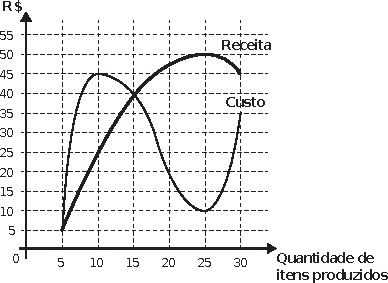
\includegraphics[width=.4\textwidth]{subareas/matematica/enem_2020-136-grafico.pdf}
\end{center}

O lucro é determinado pela diferença: Receita – Custo.

O gráfico que representa o lucro dessa empresa, em função da quantidade de itens produzidos, é

\begin{alternativas}
\setlength{\columnseprule}{0pt}
\setlength{\columnsep}{6mm}
\begin{multicols}{2}
  \item \parbox{\linewidth}{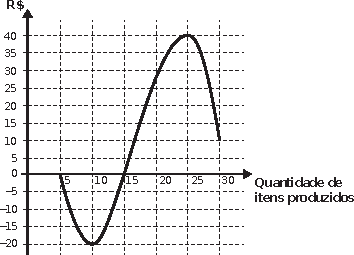
\includegraphics[width=.35\textwidth]{subareas/matematica/enem_2020-136-A.pdf}}
  \item \parbox{\linewidth}{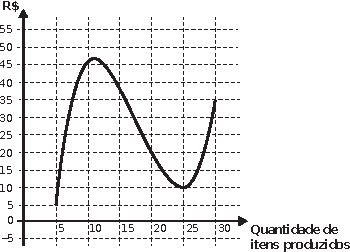
\includegraphics[width=.35\textwidth]{subareas/matematica/enem_2020-136-D.pdf}}
  \item \parbox{\linewidth}{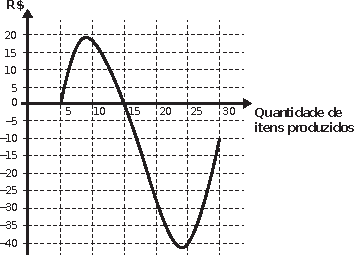
\includegraphics[width=.35\textwidth]{subareas/matematica/enem_2020-136-B.pdf}}
  \item \parbox{\linewidth}{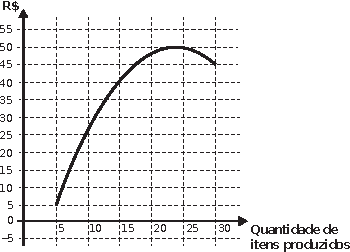
\includegraphics[width=.35\textwidth]{subareas/matematica/enem_2020-136-E.pdf}}
  \item \parbox{\linewidth}{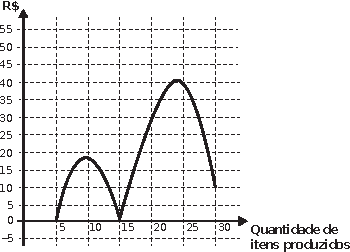
\includegraphics[width=.35\textwidth]{subareas/matematica/enem_2020-136-C.pdf}}
\end{multicols}
\end{alternativas}


\twocolumn

\questao %(ENEM - 2020)
Um motociclista planeja realizar uma viagem cujo
destino fica a 500 km de sua casa. Sua moto consome
5 litros de gasolina para cada 100 km rodados, e o
tanque da moto tem capacidade para 22 litros. Pelo
mapa, observou que no trajeto da viagem o último posto
disponível para reabastecimento, chamado Estrela, fica a
80 km do seu destino. Ele pretende partir com o tanque
da moto cheio e planeja fazer somente duas paradas para
reabastecimento, uma na ida e outra na volta, ambas no
posto Estrela. No reabastecimento para a viagem de ida,
deve considerar também combustível suficiente para se
deslocar por 200 km no seu destino.

A quantidade mínima de combustível, em litro, que
esse motociclista deve reabastecer no posto Estrela na
viagem de ida, que seja suficiente para fazer o segundo
reabastecimento, é

\begin{alternativas}
\item 13
\item 14
\item 17
\item 18
\item 21
\end{alternativas}

\questao
Uma administração municipal encomendou a pintura
de dez placas de sinalização para colocar em seu pátio
de estacionamento.

O profissional contratado para o serviço inicial
pintará o fundo de dez placas e cobrará um valor de
acordo com a área total dessas placas. O formato
de cada placa é um círculo de diâmetro $d = 40$ cm,
que tangencia lados de um retângulo, sendo que
o comprimento total da placa é $h = 60$ cm, conforme
ilustrado na figura. Use $3,14$ como aproximação para $\pi$.

\begin{center}

\includegraphics[width=.2\textwidth]{subareas/matematica/enem_2019-151-desenho.pdf}
\end{center}

Qual é a soma das medidas das áreas, em centímetros
quadrados, das dez placas?

\begin{alternativas}
\item 16 628
\item 22 280
\item 28 560
\item 41 120
\item 66 240
\end{alternativas}

\questao
O dono de um restaurante situado às margens de
uma rodovia percebeu que, ao colocar uma placa de
propaganda de seu restaurante ao longo da rodovia, as
vendas aumentaram. Pesquisou junto aos seus clientes
e concluiu que a probabilidade de um motorista perceber
uma placa de anúncio é $\displaystyle \frac{1}{2}$.
Com isso, após autorização
do órgão competente, decidiu instalar novas placas com
anúncios de seu restaurante ao longo dessa rodovia, de
maneira que a probabilidade de um motorista perceber
pelo menos uma das placas instaladas fosse superior
a $\displaystyle \frac{99}{100}$.

A quantidade mínima de novas placas de propaganda a
serem instaladas é

\begin{alternativas}
\item 99
\item 51
\item 50
\item 6
\item 1
\end{alternativas}

\questao
O colesterol total de uma pessoa é obtido pela
soma da taxa do seu “colesterol bom” com a taxa do
seu “colesterol ruim”. Os exames periódicos, realizados
em um paciente adulto, apresentaram taxa normal
de “colesterol bom”, porém, taxa do “colesterol ruim”
(também chamado LDL) de 280 mg/dL.

O quadro apresenta uma classificação de acordo com
as taxas de LDL em adultos.

\begin{center}
\begin{tabular}{|c|c|}
\hline
\multicolumn{2}{|c|}{\textbf{Taxa de LDL (mg/dL)}} \\
\hline
Ótima & Menor do que 100 \\
\hline
Próxima de ótima & De 100 a 129 \\
\hline
Limite & De 130 a 159 \\
\hline
Alta & De 160 a 189 \\
\hline
Muito alta & 190 ou mais \\
\hline
\end{tabular}
\end{center}

%\begin{flushright}
%\small Disponível em: www.minhavida.com.br. Acesso em: 15 out. 2015 (adaptado)
%\end{flushright}

O paciente, seguindo as recomendações médicas sobre estilo de vida e alimentação,
realizou o exame logo após o primeiro mês, e a taxa de LDL reduziu em $25\%$.
No mês seguinte, realizou novo exame e constatou uma redução de mais $20\%$ na taxa de LDL.

De acordo com o resultado do segundo exame, a classificação da taxa de LDL do paciente é

\begin{alternativas}
\item ótima
\item próxima de ótima
\item limite
\item alta
\item muito alta
\end{alternativas}

\questao
O Índice de Desenvolvimento Humano (IDH) é uma
medida usada para classificar os países pelo seu grau
de desenvolvimento. Para seu cálculo, são levados em
consideração a expectativa de vida ao nascer, tempo de
escolaridade e renda per capita, entre outros. O menor
valor deste índice é zero e o maior é um. Cinco países
foram avaliados e obtiveram os seguintes índices de
desenvolvimento humano: o primeiro país recebeu um
valor $X$, o segundo $\sqrt{X}$, o terceiro $\displaystyle X^{\frac{1}{3}}$,
o quarto $X^2$ e o último $X^3$. Nenhum desses países zerou ou atingiu o
índice máximo.

Qual desses países obteve o maior IDH?

\begin{alternativas}
\item O primeiro
\item O segundo
\item O terceiro
\item O quarto
\item O quinto
\end{alternativas}

\questao
Uma empresa tem diversos funcionários. Um deles
é o gerente, que recebe R\$ 1 000,00 por semana.
Os outros funcionários são diaristas. Cada um deles
trabalha 2 dias por semana, recebendo R\$ 80,00 por
dia trabalhado.

Chamando de $X$ a quantidade total de funcionários
da empresa, a quantia $Y$, em reais, que esta empresa
gasta semanalmente para pagar seus funcionários é
expressa por
\begin{alternativas}
\item $Y = 80X + 920$
\item $Y = 80X + 1000$
\item $Y = 80X + 1080$
\item $Y = 160X + 840$
\item $Y = 160X + 1000$
\end{alternativas}

\questao
Pesquisadores da Universidade de Tecnologia
de Viena, na Áustria, produziram miniaturas de
objetos em impressoras 3D de alta precisão. Ao
serem ativadas, tais impressoras lançam feixes de
laser sobre um tipo de resina, esculpindo o objeto
desejado. O produto final da impressão é uma
escultura microscópica de três dimensões, como
visto na imagem ampliada.

\begin{center}
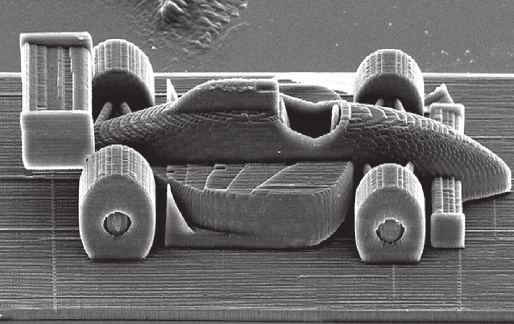
\includegraphics[width=.48\textwidth]{subareas/matematica/enem_2020-147-foto.pdf}
\end{center}

A escultura apresentada é uma miniatura de
um carro de Fórmula 1, com 100 micrômetros de
comprimento. Um micrômetro é a milionésima parte
de um metro.

Usando notação científica, qual é a representação do
comprimento dessa miniatura, em metro?

\begin{alternativas}
\item $1,0 \times 10^{-1}$
\item $1,0 \times 10^{-3}$
\item $1,0 \times 10^{-4}$
\item $1,0 \times 10^{-6}$
\item $1,0 \times 10^{-7}$
\end{alternativas}

\questao
Construir figuras de diversos tipos, apenas
dobrando e cortando papel, sem cola e sem tesoura, é
a arte do \textit{origami} (\textit{ori} = dobrar; \textit{kami} = papel), que tem
um significado altamente simbólico no Japão. A base
do origami é o conhecimento do mundo por base do
tato. Uma jovem resolveu construir um cisne usando
a técnica do \textit{origami}, utilizando uma folha de papel de
18 cm por 12 cm. Assim, começou por dobrar a folha
conforme a figura.

\begin{center}
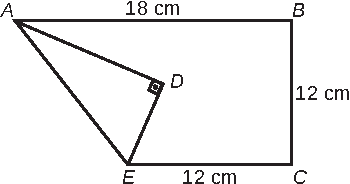
\includegraphics[width=.35\textwidth]{subareas/matematica/enem_2019-171-desenho.pdf}
\end{center}

Após essa primeira dobradura, a medida do segmento
$AE$ é

\begin{alternativas}
\item $2\sqrt{22}$ cm
\item $6\sqrt{3}$ cm
\item $12$ cm
\item $6\sqrt{5}$ cm
\item $12\sqrt{2}$ cm
\end{alternativas}

\questao \label{mat-last}
A raiva é uma doença viral e infecciosa, transmitida por mamíferos.
A campanha nacional de vacinação antirrábica tem o objetivo de controlar
a circulação do vírus da raiva canina e felina, prevenindo a raiva
humana. O gráfico mostra a cobertura (porcentagem de vacinados) da campanha, 
em cães, nos anos de 2013, 2015 e 2017, no município de Belo Horizonte,
em Minas Gerais. Os valores das coberturas dos anos de 2014 e 2016 não estão
informados no gráfico e deseja-se estimá-los. Para tal, levou-se em consideração que
a variação na cobertura de vacinação da campanha antirrábica, nos períodos
de 2013 a 2015 e de 2015 a 2017, deu-se de forma linear.

\begin{center}
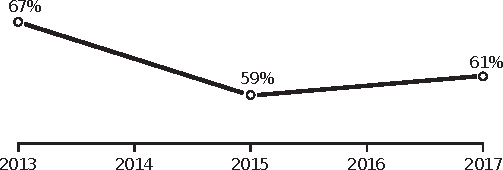
\includegraphics[width=.48\textwidth]{subareas/matematica/enem_2018-143-grafico.pdf}
\end{center}

Qual teria sido a cobertura dessa campanha no ano de 2014?

\begin{alternativas}
\item 62,3\%
\item 63,0\%
\item 63,0\%
\item 64,0\%
\item 65,5\%
\end{alternativas}


\end{document}
